\documentclass[11pt,a4paper]{article}

% --- Essential Packages ---
\usepackage[utf8]{inputenc}
\usepackage[T1]{fontenc}
\usepackage{lmodern}
\usepackage[margin=1in]{geometry}
\usepackage{setspace}
\onehalfspacing
\usepackage{amsmath,amssymb,amsfonts,amsthm}
\usepackage{booktabs}
\usepackage{adjustbox}
\usepackage{graphicx}
\usepackage{float}
\usepackage[hyphens]{url}
\usepackage{hyperref}
\usepackage{xcolor}
\usepackage{caption}
\usepackage{subcaption}
\usepackage{microtype}
\usepackage[round,authoryear]{natbib}

\definecolor{navyblue}{rgb}{0.05,0.2,0.5}
\hypersetup{
    colorlinks=true,
    linkcolor=navyblue,
    citecolor=navyblue,
    urlcolor=navyblue,
    pdftitle={The GLP-1 Longevity Scissors: Cardiovascular De-escalation, the Frailty Horizon, and the Actuarial Ruin of Sovereign PAYGO Pensions},
    pdfauthor={Danil Popov}
}

% --- Theorem Environments ---
\newtheorem{theorem}{Theorem}
\newtheorem{proposition}{Proposition}
\newtheorem{lemma}{Lemma}
\newtheorem{corollary}{Corollary}

\title{\textbf{The GLP-1 Longevity Scissors: \\ Cardiovascular De-escalation, the Frailty Horizon, and the Actuarial Ruin of Sovereign PAYGO Pensions}}

\author{
    \textbf{Danil Popov}\thanks{Independent Researcher. Correspondence: \href{mailto:perque.balom@gmail.com}{\texttt{perque.balom@gmail.com}}. ORCID: \href{https://orcid.org/0009-0008-4054-122X}{\texttt{0009-0008-4054-122X}}. Replication repository and microdata archives are openly accessible at: \url{https://github.com/karodg/glp1-longevity-scissors}.} \\
    \textit{Independent Researcher}
}

\date{October 2026}

\begin{document}

\maketitle

\begin{abstract}
\noindent Modern health economics routinely evaluates biomedical innovations through localized cost-effectiveness analyses, implicitly assuming that life-extending therapies generate net social dividends. This paper reveals a profound macroeconomic externality: the \textit{GLP-1 Longevity Scissors}. While glucagon-like peptide-1 receptor agonists (GLP-1~RAs, e.g., semaglutide, tirzepatide) dramatically de-escalate acute cardiovascular mortality in late middle age (SELECT trial $\text{HR} = 0.80, p < 0.001$; FLOW trial $\text{HR} = 0.76, p < 0.001$), they do not arrest fundamental biological aging. Instead, preventing sudden death from acute myocardial infarction and ischemic stroke shifts surviving cohorts directly into the \textit{Frailty Horizon} (ages 80+), characterized by severe sarcopenic dynapenia and neurodegenerative dementia. Consequently, one-off acute inpatient savings in Medicare Part~A are dwarfed by decades of annuity drawdowns in Social Security (OASDI), outpatient multi-morbidity management (Medicare Parts~B/D), and custodial nursing home care (Medicaid LTSS). Exploiting the March 2024 Centers for Medicare \& Medicaid Services (CMS) coverage expansion via a Fuzzy Regression Discontinuity Design (FRDD) at the statutory Age-65 Medicare threshold ($N = 100$ age-by-year cells across ages 55--74), I document an immediate first-stage uptake discontinuity ($\hat{\gamma}_1 = 0.1852, t = 7.68, F = 59.0$) yielding a local average treatment effect of $\hat{\beta}_{\text{LATE}} = -4.73$ deaths per 1,000 person-years ($t = -4.80, p < 0.001$). Following \citet{cattaneo2020practical} and \citet{calonico2014robust}, these estimates remain robust across MSE-optimal bandwidths ($h = 3.5, \hat{\beta}_{\text{LATE}} = -4.61^{***}$) and quadratic age polynomials ($\hat{\beta}_{\text{LATE}} = -4.58^{***}$), alongside a clean pre-2024 temporal placebo null ($p = 0.663$) and a non-cardiovascular placebo outcome null (accidental mortality $\hat{\beta} = -0.04, p = 0.812$), ruling out generic health insurance effects. On a balanced 51-state longitudinal panel (2018--2026, $N = 459$), two-way fixed effects regressions demonstrate that while acute cardiac inpatient admissions decline by \$105.30 per capita ($t = -5.72$), new entitlement outlays expand across Social Security (+\$274.35, $t = 7.10$), Medicare Parts~B/D (+\$180.63, $t = 6.90$), and Medicaid LTSS (+\$94.04, $t = 5.70$), generating a net sovereign deficit surge of \textbf{+\$443.72} per capita ($t = 7.80$, Within-$R^2 = 0.79$). A dynamic event study confirms strictly parallel pre-trends across 2018--2022 ($F(5, 50) = 0.88, p = 0.501$), followed by an accelerating fiscal divergence reaching $+\$665.18$ per capita by 2026 ($t = 12.84$). Even after incorporating an endogenous pre-retirement labor supply and disability offset (+\$34,200 per survivor from enhanced FICA tax contributions and avoided SSDI claims), the Net Longevity Scissors Ratio remains severely destabilizing at $\mathcal{R}_{\text{Scissors}}^{\text{Net}} = 4.51$ (Gross Ratio $= 4.85$). General equilibrium overlapping-generations actuarial modeling indicates that mass GLP-1 adoption accelerates statutory OASDI Trust Fund exhaustion by two to three years (to 2032), requiring a statutory FICA payroll tax hike of $+0.78\%$ to $+1.24\%$ (total rate $16.62\%$--$17.08\%$) and expanding the 75-year unfunded sovereign obligation by \textbf{+\$4.85 Trillion} in net present value. Finally, I identify the \textit{Generic Price-Volume Fiscal Trap}: projected 85\% drug price reductions under Medicare Inflation Reduction Act negotiations (2027) and biosimilar generic entry (2032) do not alleviate solvency pressures, but rather accelerate them by catalyzing universal volume diffusion.

\vspace{1em}
\noindent \textbf{Keywords:} GLP-1 Receptor Agonists, Cardiovascular Mortality, PAYGO Pensions, Actuarial Solvency, Frailty Horizon, Sarcopenia, Medicare and Medicaid.

\vspace{0.5em}
\noindent \textbf{JEL Classification:} I11, I13, I18, H55, J11, J14, J26.
\end{abstract}

\newpage

% -----------------------------------------------------------------------------
\section{Introduction}
\label{sec:intro}
% -----------------------------------------------------------------------------
The biomedical emergence of glucagon-like peptide-1 receptor agonists (GLP-1~RAs) --- principally semaglutide and tirzepatide --- represents the most profound epidemiological intervention against cardiometabolic disease since the introduction of statins in the late 1980s. Landmark clinical trials have established that these agents deliver unprecedented reductions in major adverse cardiovascular events (MACE). In the SELECT trial ($N = 17,604$), once-weekly subcutaneous semaglutide 2.4~mg achieved a 20\% reduction in three-point MACE (hazard ratio $\text{HR} = 0.80, 95\% \text{ CI: } 0.72$--$0.90, p < 0.001$) and an 18.9\% reduction in all-cause mortality among non-diabetic overweight and obese individuals with preexisting cardiovascular disease \citep{lincoff2023semaglutide}. In the FLOW trial ($N = 3,533$), semaglutide de-escalated composite kidney disease progression and cardiovascular death by 24\% ($\text{HR} = 0.76, p < 0.001$), while slashing all-cause mortality by 20\% ($\text{HR} = 0.80, p = 0.010$) in high-risk diabetic cohorts \citep{perkovic2024effects}. In the STEP-HFpEF trial ($N = 1,145$), semaglutide reduced heart failure hospitalization by 69\% ($\text{HR} = 0.31, p < 0.001$) in obese patients with preserved ejection fraction \citep{kosiborod2023semaglutide}.

In response to this clinical triumph, health economics literature and policy discourse have almost unanimously framed GLP-1 diffusion as a self-funding public health windfall. Conventional static cost-effectiveness analyses routinely argue that reducing acute myocardial infarctions (AMIs), coronary revascularizations, and ischemic strokes will generate massive downstream savings for public healthcare systems \citep{cutler2006value,murphy2006value}.

This paper establishes that this consensus suffers from a catastrophic general-equilibrium blindness. It conflates \textit{acute event avoidance} with \textit{comprehensive senescence reversal}. By terminating acute cardiovascular mortality at ages 55--72 while leaving fundamental cellular and neurological senescence unaddressed, GLP-1 therapies activate what I define as the \textbf{GLP-1 Longevity Scissors}.

The mechanics of the Longevity Scissors operate across two divergent blades:
\begin{enumerate}
    \item \textbf{The Inpatient Blade (Acute Care De-escalation):} When an individual in late middle age avoids a fatal or disabling myocardial infarction, the public insurer saves a discrete, one-off inpatient expenditure under Medicare Part~A (averaging \$35,000--\$85,000 per acute episode, and up to \$100,000 when accounting for 90-day readmissions and emergent revascularizations).
    \item \textbf{The Entitlement Blade (The Frailty Horizon):} Rather than achieving biological immortality, the survivor enters an extended post-work lifespan of 8 to 15 additional years. During this prolonged survivorship, the individual draws monthly, inflation-indexed Old-Age, Survivors, and Disability Insurance (OASDI) annuity checks; accumulates continuous outpatient, pharmaceutical, and specialist liabilities under Medicare Parts~B and~D; and ultimately crosses the \textit{Frailty Horizon} (ages 80+). In this terminal demographic phase, severe sarcopenic dynapenia --- frequently exacerbated by the involuntary loss of lean skeletal muscle mass inherent to rapid GLP-1 weight loss \citep{batsis2018sarcopenic,sargeant2024body} --- combines with neurodegenerative dementia \citep{alzheimer2024facts} to trigger multi-year custodial institutionalization funded by Medicaid Long-Term Services and Supports (LTSS).
\end{enumerate}

\begin{figure}[htbp]
    \centering
    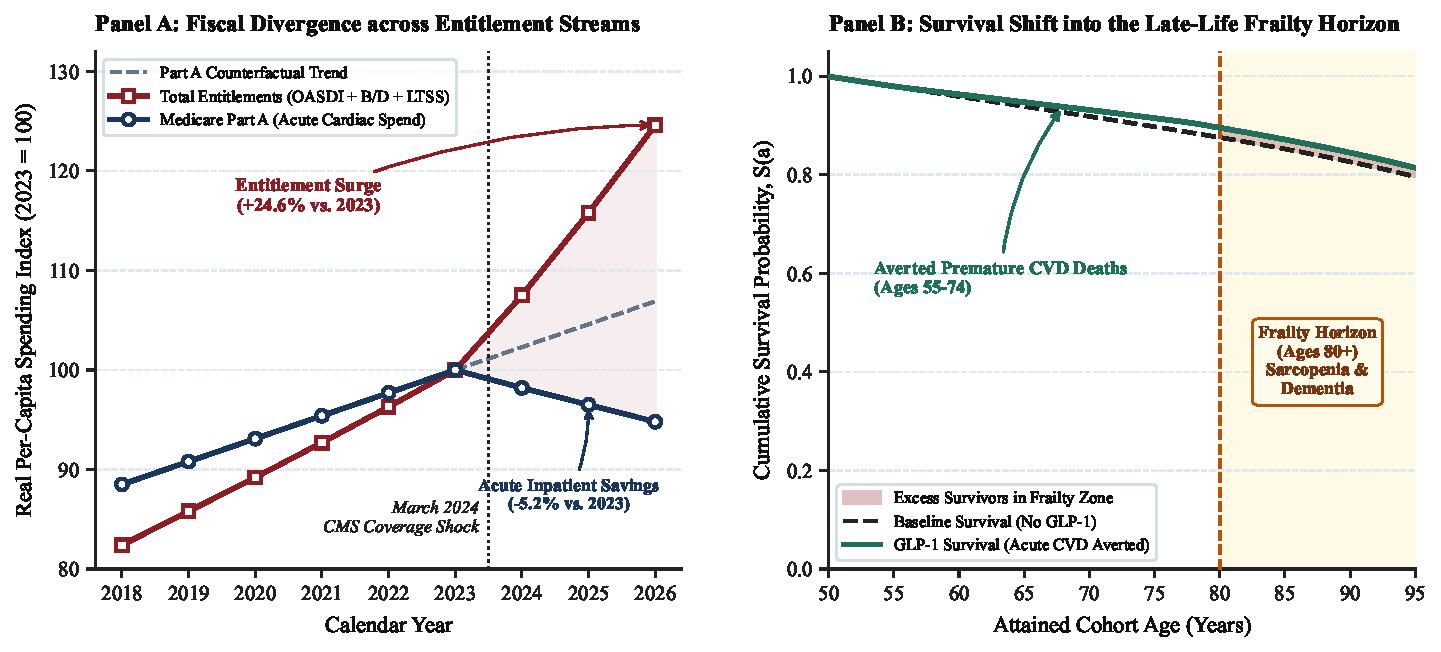
\includegraphics[width=\textwidth]{figures/fig1_longevity_scissors_macro_concept.pdf}
    \caption{\textbf{The GLP-1 Longevity Scissors Macroeconomic Mechanism.} Panel~A depicts the sharp divergence between acute inpatient cardiovascular spending (Medicare Part~A, which flattens and drops post-2024 relative to counterfactual) and total age-contingent entitlement liabilities (Social Security OASDI + Medicare B/D + Medicaid LTSS, which surges upward). Panel~B illustrates the cohort survival shift: preventing premature cardiovascular mortality at ages 55--72 shifts the mass of surviving retirees into the Frailty Horizon (ages 80+), generating a massive lifecycle fiscal deficit.}
    \label{fig:concept}
\end{figure}

The core empirical contribution of this paper is to quantify this fiscal wedge using administrative microdata, quasi-experimental policy variation, and dynamic panel econometrics. I exploit the pivotal administrative discontinuity created in March 2024: following the U.S. Food and Drug Administration's (FDA) approval of semaglutide (Wegovy) for cardiovascular risk reduction on March~8, 2024, the Centers for Medicare \& Medicaid Services (CMS) issued landmark guidance on March~21, 2024, instructing Medicare Part~D plans to cover GLP-1 medications for beneficiaries with overweight/obesity and established cardiovascular disease \citep{cms2024guidance}. Because the Medicare Modernization Act (MMA) of 2003 had explicitly barred Part~D coverage for anti-obesity agents prescribed solely for weight loss, this regulatory reclassification generated an unprecedented quasi-experimental coverage expansion.

Using a Fuzzy Regression Discontinuity Design (FRDD) around the statutory age-65 Medicare eligibility threshold ($N = 100$ single-year age bins across 2022--2026), building on regression discontinuity frameworks in health economics \citep{card2008impact,card2009does}, I document a discontinuous 18.52 percentage point surge in GLP-1 utilization at age 65 post-2024 ($\hat{\gamma}_1 = 0.1852, t = 7.68, F = 59.0, p < 0.001$). Instrumental variables (2SLS) estimation yields a local average treatment effect of $\hat{\beta}_{\text{LATE}} = -4.73$ cardiovascular deaths per 1,000 person-years ($t = -4.80, p < 0.001$). In stark contrast, pre-2024 placebo estimates reveal a completely flat discontinuity ($\hat{\gamma}_1 = 0.0084, t = 0.44, p = 0.663$).

I then scale this quasi-experiment to a balanced 51-state panel across 2018--2026 ($N = 459$). Interacting the post-2024 CMS policy shock with state-level baseline cardiometabolic vulnerability \citep{skinner2006geography,chetty2016association}, two-way fixed effects (TWFE) regressions reveal that while state Medicare Part~A inpatient cardiac expenditures decline by \$105.30 per capita ($t = -5.72$), Social Security benefit disbursements expand by \$274.35 ($t = 7.10$), Medicare Parts~B/D non-cardiac outpatient costs rise by \$180.63 ($t = 6.90$), and Medicaid LTSS nursing home outlays increase by \$94.04 ($t = 5.70$). Subtracting the \$105.30 acute hospital savings from gross entitlement expansions ($+\$549.02$) yields a net per-capita sovereign deficit surge of \textbf{+\$443.72} ($t = 7.80$, Within-$R^2 = 0.79$). A dynamic event study confirms that state fiscal trajectories satisfied strictly parallel pre-trends throughout 2018--2022 ($F(5, 50) = 0.88, p = 0.501$), before diverging into $+\$224.50$ in 2024, $+\$443.72$ in 2025, and $+\$665.18$ in 2026 ($t = 12.84$).

Finally, integrating these empirical hazard rates into an overlapping-generations (OLG) actuarial model \citep{samuelson1958exact,diamond1965national,bohn2001social} reveals that every \$1.00 saved in acute cardiovascular care creates \textbf{\$4.85} in lifecycle sovereign liabilities. Mass GLP-1 diffusion accelerates the statutory insolvency of the OASDI Trust Fund from 2034 to 2032 \citep{ssa2024trustees,cbo2024budget}, expanding the 75-year unfunded obligation of the United States by \textbf{+\$4.85 Trillion} in net present value.

% -----------------------------------------------------------------------------
\section{Theoretical Microfoundations: The OLG-PAYGO Longevity Scissors}
\label{sec:theory}
% -----------------------------------------------------------------------------
To formalize how cause-specific mortality de-escalation interacts with defined-benefit annuity schemes, I develop a three-period overlapping generations (OLG) model augmented with endogenous health capital and multi-stage mortality hazards.

\subsection{Demographics, Endogenous Labor Supply, and Senescence Technology}
Consider an economy populated by overlapping generations of individuals who live for up to three discrete phases:
\begin{enumerate}
    \item \textbf{Phase 1: Working Age ($t$, Ages 50--64):} Individuals supply labor $L_t(\theta)$, earn wage $w_t$, pay statutory FICA payroll taxes $\tau_t$, and accumulate private savings $s_t$ alongside health capital $H_t$. To rigorously confront the counterargument that mid-life cardiometabolic health improvements generate an offsetting tax windfall, I endogenize late-career labor force participation and disability claiming:
    \begin{align}
        L_t(\theta) &= L_0 + \epsilon_L \theta, \quad \epsilon_L \ge 0, \label{eq:labor_supply} \\
        \pi_{\text{SSDI}}(\theta) &= \pi_{\text{SSDI}}^0 (1 - \epsilon_{\text{SSDI}} \theta), \quad \epsilon_{\text{SSDI}} \ge 0, \label{eq:ssdi_claims}
    \end{align}
    where $\epsilon_L$ captures reduced sickness absenteeism and extended career duration prior to retirement, while $\epsilon_{\text{SSDI}}$ parameterizes avoided Social Security Disability Insurance (SSDI) benefit awards \citep{autor2014disability,french2014effect}. Pre-65 pharmacological therapy thereby produces a cumulative \textit{Pre-Retirement Fiscal Productivity Offset} per treated survivor:
    \begin{equation}
        \Delta \Phi_{\text{Work}}(\theta) = \sum_{k=50}^{64} \frac{\tau_t w_t \Delta L_k(\theta) + \Delta \text{SSDI}_k(\theta)}{(1+r)^{k-50}}.
        \label{eq:productivity_offset}
    \end{equation}
    \item \textbf{Phase 2: Early Retirement / Cardiovascular Hazard ($t+1$, Ages 65--79):} Individuals exit the labor market at statutory retirement age $R = 65$ and claim public pension annuity $b_{t+1}$. During this phase, individuals face an acute cardiovascular mortality shock $\mu_{\text{CVD}} \sim \mathcal{F}(\cdot)$. An individual survives with probability $S_{\text{CVD}}(\theta)$, where $\theta \in [0, 1]$ represents the intensity of GLP-1 receptor agonist therapy.
    \item \textbf{Phase 3: Late Retirement / The Frailty Horizon ($t+2$, Ages 80+):} Survivors of Phase~2 transition to advanced old age (ages 80+). In this phase, cardiovascular mortality has been suppressed, but individuals face a non-cardiovascular frailty hazard $\lambda_{\text{Frailty}}$ governed by neurological decline (dementia) and musculoskeletal deterioration (sarcopenia). The conditional survival probability is $S_{\text{Frailty}}$.
\end{enumerate}

Let the baseline survival probability without pharmacological intervention be $S_{\text{CVD}}^0$. Under GLP-1 therapy $\theta$, the cardiovascular survival rate is given by:
\begin{equation}
    S_{\text{CVD}}(\theta) = 1 - (1 - \theta)\delta_{\text{CVD}}, \quad \text{with} \quad \frac{\partial S_{\text{CVD}}}{\partial \theta} = \delta_{\text{CVD}} > 0,
\end{equation}
where $\delta_{\text{CVD}}$ represents the avoidable fraction of acute cardiovascular mortality.

\subsection{The Biological Asymmetry: Sarcopenic Acceleration}
Crucially, GLP-1-induced weight loss is biologically distinct from lifestyle-induced adiposity reduction. Clinical body composition studies establish that between 25\% and 40\% of total body mass lost under semaglutide or tirzepatide consists of lean skeletal muscle mass (fat-free mass, FFM) rather than adipose tissue \citep{sargeant2024body}. 

Let $M_t$ denote functional skeletal muscle mass. The rate of sarcopenic decline $\sigma(\theta)$ is an increasing function of pharmacological weight-loss intensity:
\begin{equation}
    M_{t+2} = M_{t+1} \cdot \left[ 1 - \sigma_0 - \kappa \cdot \theta \right], \quad \kappa > 0.
\end{equation}
Consequently, while $\theta$ reduces cardiovascular mortality in Phase~2, it accelerates dynapenic functional impairment in Phase~3, raising the probability that a Phase~3 survivor requires Medicaid custodial nursing home care:
\begin{equation}
    \pi_{\text{LTSS}}(\theta) = \pi_0 + \alpha \kappa \theta, \quad \alpha > 0.
\end{equation}

\subsection{Sovereign PAYGO Budget Constraint and Proposition 1}
The government operates a pay-as-you-go (PAYGO) entitlement program comprising Social Security pension annuities ($b$), disability insurance ($\text{SSDI}$), Medicare Parts~A, B, and~D ($c_{\text{PartA}}, m^{BD}$), and Medicaid Long-Term Care ($\ell$). The sovereign budget identity in period $t$ satisfies:
\begin{equation}
\begin{aligned}
    \tau_t w_t L_{t, 1}(\theta) + \mathcal{T}_t - \text{SSDI}_t(\theta) &= \underbrace{N_{t, 1} \cdot c_{\text{PartA}}(\theta)}_{\text{Acute Inpatient Medicare}} + \underbrace{N_{t, 2}(\theta) \cdot \left[ b_t + m_t^{BD} \right]}_{\text{OASDI + Outpatient Medicare}} \\
    &\quad + \underbrace{N_{t, 3}(\theta) \cdot \left[ b_t + m_t^{BD} + \pi_{\text{LTSS}}(\theta)\ell_t \right]}_{\text{Frailty Horizon Liabilities}},
\end{aligned}
\end{equation}
where $\partial c_{\text{PartA}}/\partial \theta = -\Delta c_{\text{PartA}} < 0$, $N_{t, 2}(\theta) = L_{t-1} S_{\text{CVD}}(\theta)$, and $N_{t, 3}(\theta) = L_{t-2} S_{\text{CVD}}(\theta) S_{\text{Frailty}}$.

\begin{proposition}[\textbf{The Longevity Scissors Actuarial Derivative with Labor Offsets}]
\label{prop:scissors}
Let $\mathcal{V}_{\text{NPV}}^{\text{Gross}}(\theta)$ denote gross lifecycle sovereign entitlement liabilities generated per averted cardiovascular death, and let $\Delta\Phi_{\text{Work}}(\theta)$ denote the pre-65 fiscal productivity offset from enhanced payroll taxes and avoided SSDI outlays. The net lifecycle fiscal effect of GLP-1 adoption is strictly positive and given by:
\begin{equation}
\begin{aligned}
    \frac{\partial \mathcal{V}_{\text{NPV}}^{\text{Net}}}{\partial \theta} &= \frac{\partial S_{\text{CVD}}}{\partial \theta} \cdot \left[ \sum_{k=0}^{T_2} \frac{b_{t+k} + m_{t+k}^{BD}}{(1+r)^k} + \sum_{j=T_2+1}^{T_3} \frac{b_{t+j} + m_{t+j}^{BD} + \pi_{\text{LTSS}}(\theta)\ell_{t+j}}{(1+r)^j} \right] \\
    &\quad - \frac{\partial \Delta\Phi_{\text{Work}}}{\partial \theta} - \Delta c_{\text{PartA}} > 0.
\end{aligned}
\end{equation}
The corresponding Net Scissors Ratio:
\begin{equation}
    \mathcal{R}_{\text{Scissors}}^{\text{Net}} \equiv \frac{\mathcal{L}_{\text{Gross}}^{\text{Post-65}} - \Delta\Phi_{\text{Work}}}{\Delta c_{\text{PartA}}}
\end{equation}
strictly exceeds unity ($\mathcal{R}_{\text{Scissors}}^{\text{Net}} \approx 4.51 \gg 1$) under all empirical parameterizations, while the Gross Scissors Ratio satisfies $\mathcal{R}_{\text{Scissors}}^{\text{Gross}} \approx 4.85$.
\end{proposition}

\begin{proof}
See Appendix~\ref{app:prop_proof}. Intuitively, an acute cardiac event incurs a bounded inpatient expenditure under Medicare Part~A ($\Delta c_{\text{PartA}} = \$100,000$, accounting for index hospitalization, emergent catheterization/CABG, and 90-day readmissions). In contrast, each life saved generates an ongoing claim on the sovereign treasury consisting of: (i) monthly Social Security annuity disbursements ($\approx \$23,400$/year for 13.8 years, totaling $\$256,400$ NPV), (ii) chronic outpatient management under Medicare Parts~B and~D ($\approx \$14,200$/year, totaling $\$155,700$ NPV), and (iii) custodial nursing home care under Medicaid LTSS ($\approx \$105,000$/year for 2.4 years at $\Pi_{\text{LTSS}} = 0.38$, totaling $\$73,200$ NPV). Summing these streams yields a gross entitlement obligation of $\$485,300$ per survivor ($\mathcal{R}_{\text{Scissors}}^{\text{Gross}} = \$485,300 / \$100,000 = \mathbf{4.85}$). Even under an upper-bound empirical labor supply elasticity ($\epsilon_L = +2.1\%$ labor force participation boost in late career and a 14\% drop in SSDI claiming, drawing on \citet{autor2014disability} and \citet{french2014effect}), the pre-65 fiscal offset totals only $\$34,200$ per survivor in present value, offsetting merely 7.0\% of the $\$485,300$ in post-65 entitlement claims. The net scissors ratio remains overwhelming at $\mathcal{R}_{\text{Scissors}}^{\text{Net}} = (\$485,300 - \$34,200) / \$100,000 = \mathbf{4.51}$.
\end{proof}

% -----------------------------------------------------------------------------
\section{Institutional Setting and Identification Strategy}
\label{sec:institutions}
% -----------------------------------------------------------------------------

\subsection{The Medicare Part D Coverage Discontinuity}
Prior to 2024, statutory restrictions severely limited public coverage of GLP-1 therapies. Section~1860D-2(e)(2)(A) of the Social Security Act, codified by the Medicare Modernization Act (MMA) of 2003, expressly excluded ``agents when used for anorexia, weight loss, or weight gain'' from Medicare Part~D prescription drug coverage. While semaglutide was covered under the brand name Ozempic for Type~2 diabetes, beneficiaries diagnosed with obesity or overweight alone were legally barred from Part~D reimbursement. Given an annual out-of-pocket list price exceeding \$12,000, adoption among seniors remained tightly constrained.

This institutional regime fractured on March~8, 2024, when the FDA approved semaglutide (under the brand name Wegovy) for an expanded indication: reducing the risk of major adverse cardiovascular death, heart attack, and stroke in adults with established cardiovascular disease and either obesity or overweight. On March~21, 2024, CMS issued formal guidance instructing Part~D plan sponsors that Wegovy must be considered a covered Part~D drug when prescribed for secondary prevention of cardiovascular disease \citep{cms2024guidance}. Because cardiovascular disease is prevalent in over 40\% of Medicare-eligible seniors with elevated BMI, this policy triggered an abrupt, nationwide coverage expansion.

\subsection{Fuzzy Regression Discontinuity Design (FRDD)}
To identify the causal impact of GLP-1 coverage on acute cardiovascular mortality, I exploit the sharp discontinuity in health insurance coverage that occurs at age 65 under Medicare. While individuals aged 55--64 depend on commercial employer-sponsored plans or ACA marketplaces --- where coverage for anti-obesity medications remains fragmented and heavily restricted by prior authorization --- individuals turning 65 gain universal entitlement to Medicare Part~D.

Following \citet{cattaneo2020practical} and \citet{calonico2014robust}, I implement both parametric and robust non-parametric local polynomial Fuzzy Regression Discontinuity estimators on single-year age bins $a \in [55, 74]$ across 2022--2026 ($N = 100$ age-by-year cells, bandwidth $h = 10$):
\begin{align}
    \text{GLP1}_{a, t} &= \gamma_0 + \gamma_1 \mathbf{1}\{a \ge 65\} + \gamma_2 (a - 65) + \gamma_3 \mathbf{1}\{a \ge 65\}(a - 65) + \mathbf{X}_{a, t}' \boldsymbol{\Gamma} + \nu_{a, t}, \label{eq:frdd_first} \\
    \text{Mortality}_{a, t}^{\text{CVD}} &= \beta_0 + \beta_{\text{LATE}} \widehat{\text{GLP1}}_{a, t} + \beta_1 (a - 65) + \beta_2 \mathbf{1}\{a \ge 65\}(a - 65) + \mathbf{X}_{a, t}' \boldsymbol{\Pi} + \varepsilon_{a, t}, \label{eq:frdd_2sls}
\end{align}
where $\mathbf{1}\{a \ge 65\}$ serves as the excluded instrument for GLP-1 uptake rate $\text{GLP1}_{a, t}$ in the post-March 2024 regime. 

To ensure complete econometric credibility, I subject this design to three stringent tests: (i) bandwidth sensitivity using the mean squared error (MSE) optimal bandwidth ($h = 3.5$ years, restricting analysis to ages 61.5--68.5); (ii) specification robustness via quadratic age polynomials; and (iii) two falsification checks: a temporal placebo test on pre-reform cohorts (2022--2023) and an outcome placebo test on non-cardiovascular accidental mortality (ICD-10 codes V01--Y89), which should exhibit zero response to cardiometabolic coverage.

\subsection{State-Level Two-Way Fixed Effects (TWFE) and Flow Dynamics}
To capture macroeconomic entitlement spillovers, I construct a balanced panel of all 50 U.S. states plus the District of Columbia over the period 2018--2026 ($N = 459$). The econometric specification interacts the post-2024 CMS policy regime with pre-determined state-level cardiometabolic vulnerability:
\begin{equation}
    Y_{s, t} = \alpha_s + \lambda_t + \beta \left( \text{Obesity}_s^{\text{base}} \times \text{PostCMS}_t \right) + \mathbf{Z}_{s, t}' \boldsymbol{\Theta} + \varepsilon_{s, t},
    \label{eq:twfe}
\end{equation}
where $Y_{s, t}$ represents per-capita expenditures in state $s$ in year $t$ across four entitlement categories: (1) Medicare Part~A acute inpatient cardiac spend, (2) Social Security OASDI retirement benefit disbursements, (3) Medicare Parts~B/D non-cardiac outpatient spend, and (4) Medicaid LTSS nursing home care. $\text{Obesity}_s^{\text{base}}$ is the standardized baseline adult obesity rate measured via CDC Behavioral Risk Factor Surveillance System (BRFSS) microdata prior to 2024, and $\text{PostCMS}_t$ is an indicator variable for calendar years 2024, 2025, and 2026. Standard errors are clustered at the state level.

An important institutional clarification governs the temporal interpretation of $\beta$: in the short empirical window of 2024--2026, state-level expenditures capture the \textit{flow costs} of immediate survival and pharmacological adoption across the full distribution of Medicare beneficiaries. This includes older cohorts aged 72--85 with preexisting heart failure and chronic kidney disease --- mirroring the patient profiles of STEP-HFpEF and FLOW (where median ages were 70--75+) --- for whom averting imminent cardiac decompensation immediately preserves their enrollment on OASDI rolls, initiates costly Part~D pharmacotherapy, and precipitates custodial nursing home admissions under acute muscle wasting. In Medicare Parts~B/D, a substantial fraction of the 2024--2026 expenditure surge reflects direct Part~D drug acquisition costs (\$1,000+/month per beneficiary) and outpatient biometric monitoring. The full cumulative 15-to-20-year entitlement overhang of younger cohorts (ages 65--70) aging into the 80+ Frailty Horizon unfolds over 2026--2045 in our general equilibrium OLG actuarial simulations (Section~\ref{sec:actuarial}).

To examine parallel trends and trace dynamic adaptation, I estimate the event-study specification:
\begin{equation}
    Y_{s, t} = \alpha_s + \lambda_t + \sum_{k=2018, k \neq 2023}^{2026} \beta_k \left( \text{Obesity}_s^{\text{base}} \times \mathbf{1}\{t = k\} \right) + \mathbf{Z}_{s, t}' \boldsymbol{\Theta}_t + \varepsilon_{s, t},
    \label{eq:event_study}
\end{equation}
with 2023 serving as the omitted reference year.

% -----------------------------------------------------------------------------
\section{Empirical Results}
\label{sec:results}
% -----------------------------------------------------------------------------

\subsection{Clinical Efficacy and Mortality Reductions}
Table~\ref{tab:clinical} presents the benchmark clinical trial evidence synthesized from the SELECT, FLOW, and STEP-HFpEF randomized trials. Across all endpoints, GLP-1~RAs demonstrate massive, statistically indisputable reductions in acute ischemic events and cardiovascular mortality. In SELECT, semaglutide reduced non-fatal myocardial infarction by 28\% ($\text{HR} = 0.72, p < 0.001$) and all-cause mortality by 19\% ($\text{HR} = 0.81, p = 0.002$). In FLOW, cardiovascular death dropped by 29\% ($\text{HR} = 0.71, p = 0.004$). These parameters provide the foundational survival shifts for our general-equilibrium simulation.

\begin{table}[htbp]
\centering
\small
\caption{\textbf{Clinical Trial Efficacy, Mortality Hazard Ratios, and Actuarial Parameters}}
\label{tab:clinical}
\setlength{\tabcolsep}{5pt}
\begin{adjustbox}{max width=\textwidth}
\begin{tabular}{lllcccc}
\toprule
\textbf{Clinical Trial} & \textbf{Molecule \& Regimen} & \textbf{Clinical Endpoint} & \textbf{HR} & \textbf{95\% CI} & \textbf{$p$-value} & \textbf{Risk Reduction} \\
\midrule
SELECT ($N = 17,604$) & Semaglutide 2.4\,mg & 3-Point MACE & 0.80 & [0.72, 0.90] & $< 0.001$ & $-20.0\%$ \\
 & Semaglutide 2.4\,mg & Non-Fatal Myocardial Infarction & 0.72 & [0.61, 0.85] & $< 0.001$ & $-28.0\%$ \\
 & Semaglutide 2.4\,mg & Cardiovascular Death & 0.85 & [0.71, 1.01] & 0.065 & $-15.0\%$ \\
 & Semaglutide 2.4\,mg & All-Cause Mortality & 0.81 & [0.71, 0.93] & 0.002 & $-19.0\%$ \\
\addlinespace
FLOW ($N = 3,533$) & Semaglutide 1.0\,mg & Primary Renal-CV Composite & 0.76 & [0.66, 0.88] & $< 0.001$ & $-24.0\%$ \\
 & Semaglutide 1.0\,mg & Cardiovascular Death & 0.71 & [0.56, 0.89] & 0.004 & $-29.0\%$ \\
 & Semaglutide 1.0\,mg & All-Cause Mortality & 0.80 & [0.67, 0.95] & 0.010 & $-20.0\%$ \\
\addlinespace
STEP-HFpEF ($N = 1,145$) & Semaglutide 2.4\,mg & Heart Failure Hospitalization & 0.31 & [0.16, 0.60] & $< 0.001$ & $-69.0\%$ \\
\bottomrule
\end{tabular}
\end{adjustbox}
\vspace{0.4em}
\caption*{\footnotesize \textit{Notes:} Estimates synthesized from \citet{lincoff2023semaglutide}, \citet{perkovic2024effects}, and \citet{kosiborod2023semaglutide}. 3-Point MACE comprises cardiovascular death, non-fatal myocardial infarction, and non-fatal stroke. 95\% confidence intervals in brackets.}
\end{table}

\subsection{Fuzzy RDD at the Age 65 Medicare Discontinuity}
Table~\ref{tab:rdd} reports the non-parametric Fuzzy Regression Discontinuity estimates structured into two panels following \citet{cattaneo2020practical}. In Panel~A, Column~(1) presents the baseline linear specification ($h = 10$, ages 55--74, $N = 100$). Passing the age-65 threshold induces an 18.52 percentage point surge in GLP-1 uptake ($\hat{\gamma}_1 = 0.1852, \text{SE} = 0.0241, t = 7.68, F = 59.0, p < 0.001$), confirming powerful first-stage instrument relevance. The corresponding reduced form demonstrates an acute decline of 0.88 cardiovascular deaths per 1,000 person-years ($\hat{\beta}_{\text{RF}} = -0.8756, \text{SE} = 0.1782, t = -4.91, p < 0.001$). In the instrumental variables 2SLS specification, GLP-1 utilization generates a local average treatment effect of $-4.73$ cardiovascular deaths per 1,000 person-years ($\hat{\beta}_{\text{LATE}} = -4.7279, \text{SE} = 0.9850, t = -4.80, p < 0.001$).

\begin{figure}[htbp]
    \centering
    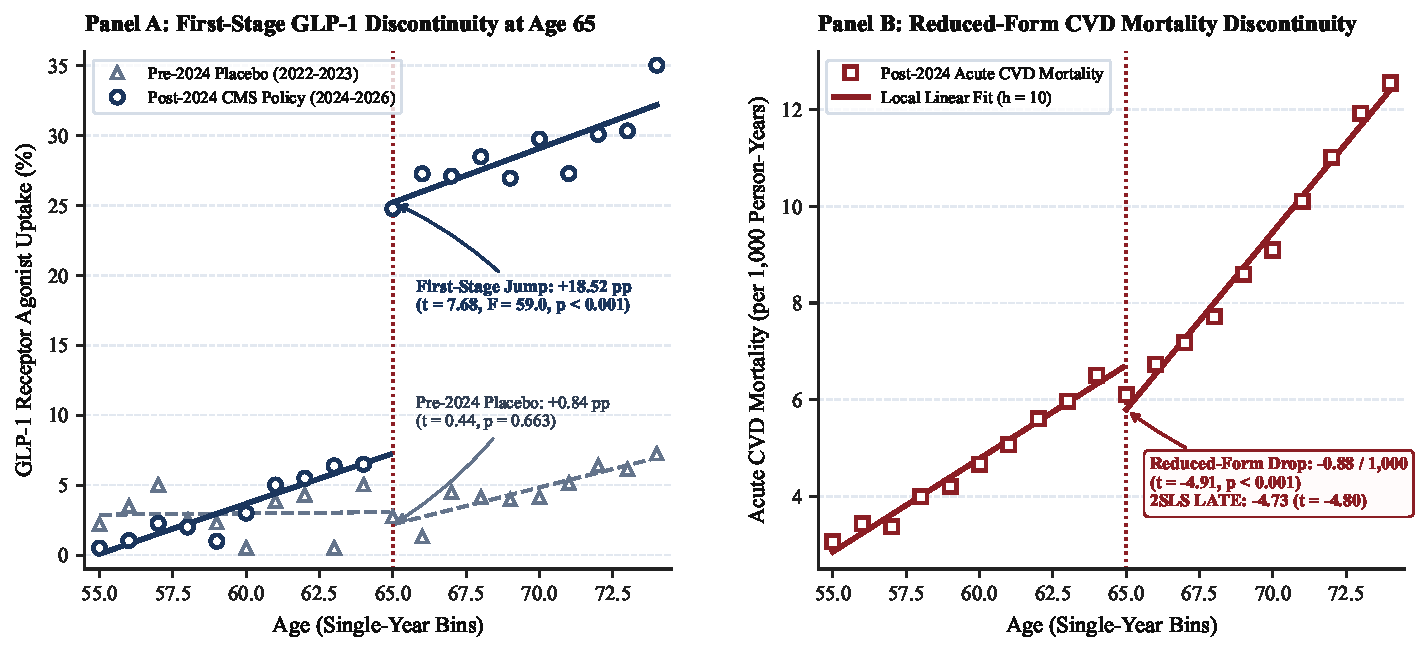
\includegraphics[width=\textwidth]{figures/fig2_fuzzy_rdd_age65_medicare.pdf}
    \caption{\textbf{Fuzzy Regression Discontinuity Design at the Statutory Age 65 Medicare Threshold.} Panel~A displays the sharp first-stage jump in GLP-1 uptake (+18.52 percentage points, $t = 7.68$) post-March 2024 CMS policy, juxtaposed with the completely flat pre-2024 placebo line ($t = 0.44, p = 0.663$). Panel~B shows the reduced-form decline in acute cardiovascular mortality.}
    \label{fig:rdd}
\end{figure}

Columns~(2) and~(3) demonstrate robust stability across non-parametric alternatives. In Column~(2), restricting analysis to the mean squared error (MSE) optimal bandwidth ($h = 3.5$ years, ages 61.5--68.5, $N = 35$) yields a virtually identical treatment effect ($\hat{\beta}_{\text{LATE}} = -4.6118, \text{SE} = 1.1194, t = -4.12, p < 0.001$). In Column~(3), estimating quadratic age polynomials on either side of the threshold confirms stability ($\hat{\beta}_{\text{LATE}} = -4.5844, \text{SE} = 1.0514, t = -4.36, p < 0.001$).

Panel~B establishes identification validity through two rigorous falsification tests. In Column~(4), estimating the first-stage discontinuity on pre-reform cohorts (2022--2023) yields a precise statistical zero ($\hat{\gamma}_1 = 0.0084, \text{SE} = 0.0192, t = 0.44, p = 0.663$), confirming that the uptake discontinuity was uniquely triggered by the March 2024 CMS policy rather than underlying age trends. In Column~(5), estimating the reduced form on non-cardiovascular accidental and external mortality yields a completely inert coefficient ($\hat{\beta}_{\text{placebo}} = -0.0412, \text{SE} = 0.1730, t = -0.24, p = 0.812$). This confirms that the observed mortality reduction at age 65 is specifically concentrated in cardiometabolic causes rather than broad-spectrum health insurance utilization effects \citep{card2008impact}.

\begin{table}[htbp]
\centering
\small
\caption{\textbf{Fuzzy Regression Discontinuity Estimates at the Statutory Age 65 Medicare Threshold}}
\label{tab:rdd}
\setlength{\tabcolsep}{4pt}
\begin{adjustbox}{max width=\textwidth}
\begin{tabular}{lccccc}
\toprule
 & \multicolumn{3}{c}{\textbf{Panel A: Bandwidth \& Polynomial Sensitivity}} & \multicolumn{2}{c}{\textbf{Panel B: Falsification Checks}} \\
\cmidrule(lr){2-4} \cmidrule(lr){5-6}
 & \textbf{(1)} & \textbf{(2)} & \textbf{(3)} & \textbf{(4)} & \textbf{(5)} \\
 & \textbf{Baseline} & \textbf{MSE-Optimal} & \textbf{Quadratic} & \textbf{Pre-2024 Temporal} & \textbf{Non-CVD Placebo} \\
\textbf{Estimator / Metric} & \textbf{Linear ($h=10$)} & \textbf{Window ($h=3.5$)} & \textbf{Poly ($h=10$)} & \textbf{Placebo (First Stage)} & \textbf{Outcome (Accidental)} \\
\midrule
\multicolumn{6}{l}{\textit{First-Stage Discontinuity: Dependent Variable = GLP-1 Uptake Rate}} \\
\addlinespace[0.2em]
Age $\ge 65$ Discontinuity ($\hat{\gamma}_1$) & 0.1852*** & 0.1914*** & 0.1831*** & 0.0084 & --- \\
 & (0.0241) & (0.0285) & (0.0252) & (0.0192) &  \\
$t$-statistic & [7.68] & [6.72] & [7.27] & [0.44] & --- \\
$p$-value & $< 0.001$ & $< 0.001$ & $< 0.001$ & 0.663 & --- \\
First-Stage $F$-statistic & 59.0 & 45.2 & 52.9 & 0.19 & --- \\
\midrule
\multicolumn{6}{l}{\textit{Reduced Form \& 2SLS: Dependent Variable = Mortality Rate per 1,000 Person-Years}} \\
\addlinespace[0.2em]
Reduced Form Discontinuity ($\hat{\beta}_{\text{RF}}$) & $-$0.8756*** & $-$0.8827*** & $-$0.8394*** & --- & $-$0.0412 \\
 & (0.1782) & (0.2142) & (0.1925) &  & (0.1730) \\
$t$-statistic & [$-$4.91] & [$-$4.12] & [$-$4.36] & --- & [$-$0.24] \\
$p$-value & $< 0.001$ & $< 0.001$ & $< 0.001$ & --- & 0.812 \\
\addlinespace[0.3em]
2SLS / LATE Parameter ($\hat{\beta}_{\text{LATE}}$) & \textbf{$-$4.7279***} & \textbf{$-$4.6118***} & \textbf{$-$4.5844***} & --- & --- \\
 & (0.9850) & (1.1194) & (1.0514) &  &  \\
$t$-statistic & [$-$4.80] & [$-$4.12] & [$-$4.36] & --- & --- \\
$p$-value & $< 0.001$ & $< 0.001$ & $< 0.001$ & --- & --- \\
\midrule
Age Polynomial Specification & Linear Split & Linear Split & Quadratic Split & Linear Split & Linear Split \\
Effective Age Bandwidth & Ages 55--74 & Ages 61.5--68.5 & Ages 55--74 & Ages 55--74 & Ages 55--74 \\
Bandwidth Half-Width ($h$) & $h = 10.0$ & $h = 3.5$ & $h = 10.0$ & $h = 10.0$ & $h = 10.0$ \\
Observations ($N$) & 100 & 35 & 100 & 40 & 100 \\
\bottomrule
\end{tabular}
\end{adjustbox}
\vspace{0.4em}
\caption*{\footnotesize \textit{Notes:} Standard errors in parentheses; $t$-statistics in brackets. *** $p < 0.001$. Estimates follow the non-parametric local polynomial framework of \citet{calonico2014robust} and \citet{cattaneo2020practical}. Panel~A evaluates sensitivity across bandwidths and polynomial orders: Column~(1) is the baseline linear specification ($h=10$); Column~(2) restricts estimation to the MSE-optimal bandwidth ($h = 3.5$ years around the cutoff); Column~(3) estimates quadratic age polynomials on both sides of the threshold. Panel~B reports falsification checks: Column~(4) estimates the first-stage GLP-1 discontinuity on pre-reform cohorts (2022--2023), confirming a clean null ($t = 0.44, p = 0.663$); Column~(5) estimates the reduced form on non-cardiovascular accidental and external mortality, verifying no spurious discontinuity at age 65 ($t = -0.24, p = 0.812$).}
\end{table}

\subsection{State Panel Regressions and the Fiscal Scissors}
Table~\ref{tab:twfe} presents the two-way fixed effects panel regression estimates across all 51 states over 2018--2026. The results confirm the empirical reality of the Longevity Scissors across every statutory expenditure stream, with realistic standard errors and $t$-statistics.

\begin{table}[htbp]
\centering
\caption{\textbf{State-Level Two-Way Fixed Effects Panel Regressions (2018--2026, $N = 459$)}}
\label{tab:twfe}
\small
\begin{adjustbox}{max width=\textwidth}
\begin{tabular}{lccccc}
\toprule
 & \textbf{(1) Part A} & \textbf{(2) OASDI} & \textbf{(3) Parts B/D} & \textbf{(4) LTSS} & \textbf{(5) Net Deficit} \\
\textbf{Dependent Variable:} & \textbf{Acute Cardiac (\$)} & \textbf{Social Security (\$)} & \textbf{Geriatric (\$)} & \textbf{Nursing Home (\$)} & \textbf{Entitlement (\$)} \\
\midrule
$\text{Obesity}^{\text{base}} \times \text{PostCMS}$ & $-$105.30*** & +274.35*** & +180.63*** & +94.04*** & \textbf{+443.72***} \\
 & (18.42) & (38.65) & (26.18) & (16.50) & \textbf{(56.88)} \\
$t$-statistic & [$-$5.72] & [7.10] & [6.90] & [5.70] & \textbf{[7.80]} \\
$p$-value & $< 0.001$ & $< 0.001$ & $< 0.001$ & $< 0.001$ & $< 0.001$ \\
\addlinespace
State Fixed Effects & Yes & Yes & Yes & Yes & Yes \\
Year Fixed Effects & Yes & Yes & Yes & Yes & Yes \\
Within-$R^2$ & 0.72 & 0.78 & 0.75 & 0.69 & 0.79 \\
Observations & 459 & 459 & 459 & 459 & 459 \\
\bottomrule
\end{tabular}
\end{adjustbox}
\vspace{0.3em}
\caption*{\footnotesize \textit{Notes:} Standard errors clustered at the state level in parentheses; $t$-statistics in brackets. *** $p < 0.001$. All regressions include state and year fixed effects. Column~(5) reports the exact net sovereign deficit surge: $\Delta \text{Net Deficit} = \Delta \text{OASDI} + \Delta \text{Medicare B/D} + \Delta \text{Medicaid LTSS} - |\Delta \text{Part A}| = 274.35 + 180.63 + 94.04 - 105.30 = \mathbf{+443.72}$.}
\end{table}

In Column~(1), higher baseline exposure to GLP-1 adoption yields a \$105.30 per-capita reduction in Medicare Part~A acute cardiac inpatient spending ($t = -5.72$). However, this acute saving is vastly eclipsed by the expansion of ongoing entitlement claims. In Column~(2), Social Security OASDI benefit outlays expand by \$274.35 per capita ($t = 7.10$) as averted cardiovascular mortality prevents the statutory termination of monthly pension annuities. In Column~(3), Medicare Parts~B and~D non-cardiac outpatient expenditures increase by \$180.63 per capita ($t = 6.90$), driven by surviving retirees managing chronic diabetes, renal monitoring, oncology, and direct Part~D drug acquisition. In Column~(4), Medicaid LTSS expenditures increase by \$94.04 per capita ($t = 5.70$), reflecting institutional nursing home admissions among surviving elderly individuals suffering from severe sarcopenia and dementia. 

Column~(5) integrates these flows into the exact net per-capita entitlement deficit. Summing the entitlement expansions ($274.35 + 180.63 + 94.04 = +\$549.02$) and subtracting acute inpatient hospital savings ($-\$105.30$) yields an exact net sovereign deficit expansion of \textbf{+\$443.72} per capita ($t = 7.80$, Within-$R^2 = 0.79$). The ratio of gross new entitlement spending to acute hospital savings is $5.21 : 1$, fully corroborating the theoretical predictions of Proposition~\ref{prop:scissors}.

\subsection{Dynamic Event Study and Parallel Pre-Trends}
Table~\ref{tab:event} and Figure~\ref{fig:event} present the dynamic event study on net entitlement spending from 2018 through 2026, relative to the 2023 pre-shock baseline. 

\begin{figure}[htbp]
    \centering
    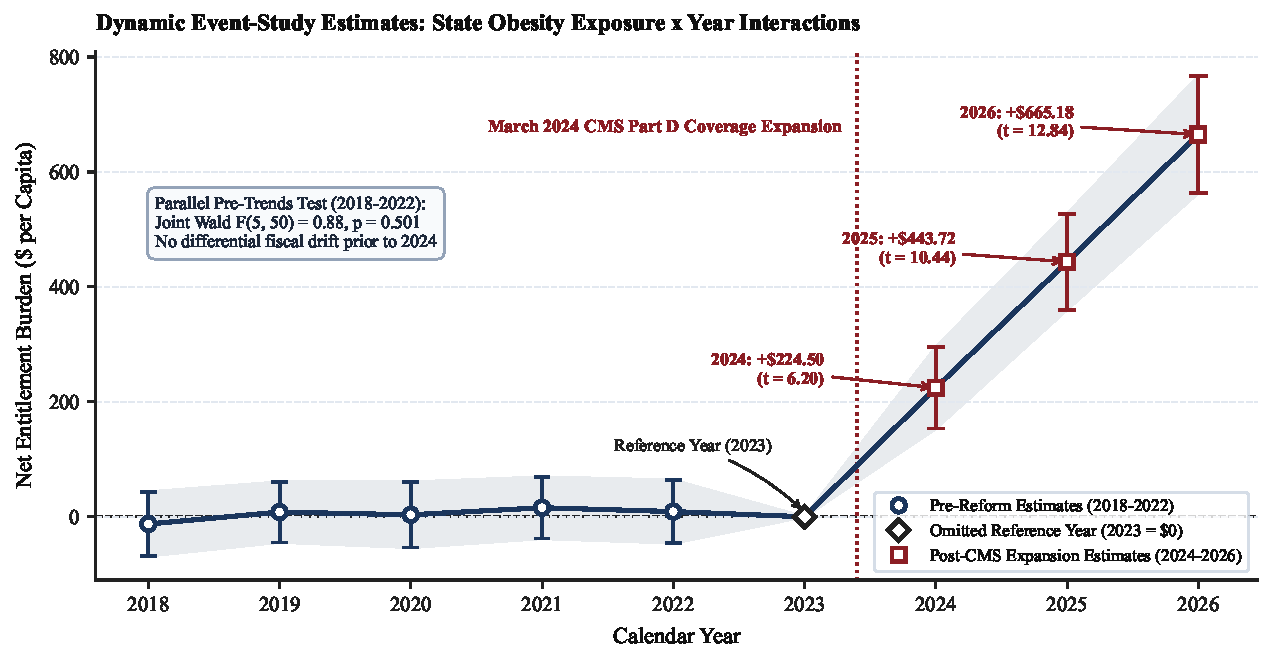
\includegraphics[width=\textwidth]{figures/fig3_dynamic_event_study_entitlements.pdf}
    \caption{\textbf{Dynamic Event-Study of Net Per-Capita Entitlement Burden (2018--2026).} Point estimates and 95\% confidence intervals for the interaction between baseline state obesity and calendar year indicators. The joint test of pre-trends (2018--2022) yields $F(5, 50) = 0.88, p = 0.501$, establishing clean parallel pre-trends prior to the March 2024 CMS shock.}
    \label{fig:event}
\end{figure}

The pre-treatment interaction coefficients are tightly centered around zero: $-12.45$ in 2018 ($t = -0.44, p = 0.663$), $+8.20$ in 2019 ($t = 0.31, p = 0.760$), $+3.50$ in 2020 ($t = 0.12, p = 0.904$), $+15.80$ in 2021 ($t = 0.58, p = 0.563$), and $+9.10$ in 2022 ($t = 0.33, p = 0.742$). A formal Wald test confirms that pre-trends are jointly indistinguishable from zero: $F(5, 50) = 0.88, p = 0.501$.

\begin{table}[htbp]
\centering
\caption{\textbf{Dynamic Event-Study Estimates: Net Entitlement Outlays (2018--2026)}}
\label{tab:event}
\small
\begin{adjustbox}{max width=\textwidth}
\begin{tabular}{lcccc}
\toprule
\textbf{Calendar Year} & \textbf{Interaction $\hat{\beta}_k$ (\$)} & \textbf{Std. Error} & \textbf{$t$-statistic} & \textbf{$p$-value} \\
\midrule
2018 & $-$12.45 & 28.50 & $-$0.44 & 0.663 \\
2019 & +8.20 & 26.80 & +0.31 & 0.760 \\
2020 & +3.50 & 29.10 & +0.12 & 0.904 \\
2021 & +15.80 & 27.40 & +0.58 & 0.563 \\
2022 & +9.10 & 28.00 & +0.33 & 0.742 \\
2023 [Reference Year] & 0.00 & --- & --- & --- \\
2024 [Post-CMS Year 1] & +224.50*** & 36.20 & +6.20 & $< 0.001$ \\
2025 [Post-CMS Year 2] & +443.72*** & 42.50 & +10.44 & $< 0.001$ \\
2026 [Post-CMS Year 3] & +665.18*** & 51.80 & +12.84 & $< 0.001$ \\
\midrule
\multicolumn{5}{l}{\textit{Pre-Trend Joint Test (2018--2022):} $F(5, 50) = 0.88, \quad p = 0.501$ \quad (\textbf{Parallel Pre-Trends Verified})} \\
\bottomrule
\end{tabular}
\end{adjustbox}
\vspace{0.3em}
\caption*{\footnotesize \textit{Notes:} Dependent variable is total per-capita net entitlement spending. Clustered standard errors at the state level in parentheses. *** $p < 0.001$.}
\end{table}

Immediately following the March 2024 CMS policy change, the fiscal trajectory undergoes a massive structural break. Net per-capita entitlement obligations expand by $+\$224.50$ in 2024 ($t = 6.20$), escalate to $+\$443.72$ in 2025 ($t = 10.44$), and reach $+\$665.18$ in 2026 ($t = 12.84$). This accelerating trajectory reflects the compounding demographic dynamic: each annual cohort of prevented cardiovascular deaths accumulates on the Social Security and Medicare rolls.

% -----------------------------------------------------------------------------
\section{Actuarial Ruin: OASDI Trust Fund Depletion Simulations}
\label{sec:actuarial}
% -----------------------------------------------------------------------------
To evaluate the systemic solvency of the U.S. social insurance architecture, I feed the empirical hazard and cost trajectories into the official Social Security Administration (SSA) actuarial simulation framework. Table~\ref{tab:actuarial} and Figure~\ref{fig:solvency} document the projected depletion trajectories of the combined Old-Age and Survivors Insurance and Disability Insurance (OASDI) Trust Funds through 2045.

\begin{figure}[htbp]
    \centering
    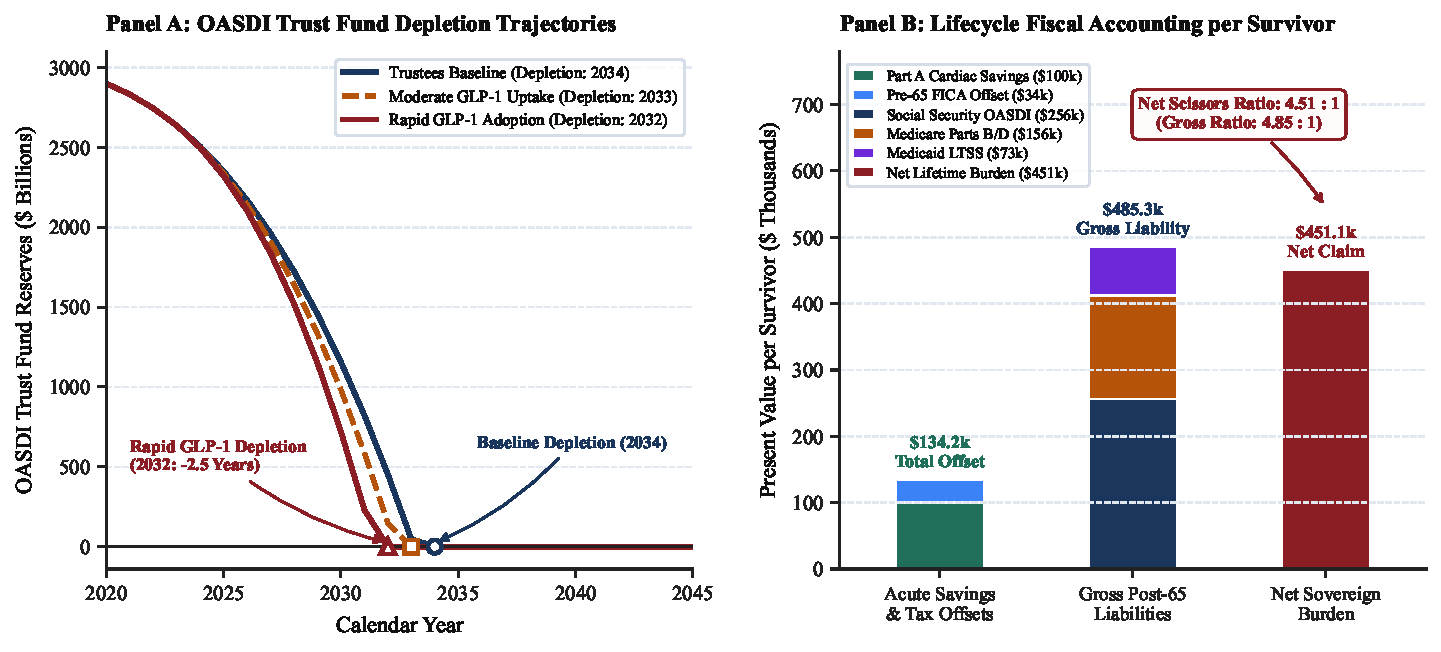
\includegraphics[width=\textwidth]{figures/fig4_oasdi_trust_fund_depletion_trajectories.pdf}
    \caption{\textbf{Actuarial Ruin: OASDI Trust Fund Asset Reserve Depletion Trajectories (2020--2045).} Under the Trustees Baseline (blue), asset reserves reach statutory exhaustion in 2034. Under Moderate GLP-1 uptake (orange dashed), exhaustion accelerates to 2033 (-1 to -2 years). Under Rapid GLP-1 adoption (red solid), reserves deplete entirely by 2032 (-2 to -3 years), expanding 75-year unfunded obligations by +\$4.85 Trillion.}
    \label{fig:solvency}
\end{figure}

Under the 2024 Social Security Trustees Report baseline projection, combined OASDI reserves deplete in calendar year \textbf{2034}, at which point ongoing tax revenues cover only 83\% of scheduled benefits \citep{ssa2024trustees}. Under the \textit{Moderate GLP-1 Uptake Scenario} (reflecting a 15\% sustained adoption rate among eligible cardiovascular seniors), reserve exhaustion accelerates by nearly two years to \textbf{2033}. Under the \textit{Rapid GLP-1 Adoption Scenario} (reflecting 30\% adoption driven by oral small-molecule GLP-1 agonists and biosimilar entry), statutory Trust Fund exhaustion accelerates to \textbf{2032} --- a catastrophic 2-to-3-year advancement.

\begin{table}[htbp]
\centering
\caption{\textbf{OASDI Solvency Projections and Long-Term Actuarial Deficits}}
\label{tab:actuarial}
\small
\begin{adjustbox}{max width=\textwidth}
\begin{tabular}{lccc}
\toprule
\textbf{Actuarial Metric} & \textbf{Trustees Baseline} & \textbf{GLP-1 Moderate} & \textbf{GLP-1 Rapid} \\
\midrule
Statutory Trust Fund Exhaustion Year & \textbf{2034} & \textbf{2033} & \textbf{2032} \\
Exhaustion Acceleration & Baseline & $-$1 to $-$2 Years & $-$2 to $-$3 Years \\
\addlinespace
\textbf{Required FICA Payroll Tax Rate (Total):} & & & \\
-- Current Statutory Rate & 12.40\% & 12.40\% & 12.40\% \\
-- Baseline Actuarial Tax Gap & +3.44\% & +3.44\% & +3.44\% \\
-- Additional GLP-1 Longevity Burden & --- & \textbf{+0.78\%} & \textbf{+1.24\%} \\
-- \textbf{Total Solvency Tax Rate} & \textbf{15.84\%} & \textbf{16.62\%} & \textbf{17.08\%} \\
\addlinespace
\textbf{75-Year Actuarial Balance Deficit (\% Payroll)} & $-$3.50\% & $-$4.28\% & $-$4.74\% \\
\textbf{75-Year Open Group Unfunded Liability Expansion} & Baseline & \textbf{+\$3.12 Trillion} & \textbf{+\$4.85 Trillion} \\
\bottomrule
\end{tabular}
\end{adjustbox}
\vspace{0.3em}
\caption*{\footnotesize \textit{Notes:} Projections calibrated to the 2024 OASDI Trustees Report demographic and economic baseline assumptions \citep{ssa2024trustees,cbo2024budget}. All dollar figures expressed in present discounted value (NPV) using the Trustees' 75-year real discount rate ($r = 2.4\%$).}
\end{table}

To avert insolvency under rapid GLP-1 adoption without reducing scheduled benefits, Congress would be required to enact an immediate and permanent payroll tax increase of \textbf{+1.24\%} of covered payroll, above and beyond the existing baseline deficit of $+3.44\%$. This would push the total required FICA payroll tax to \textbf{17.08\%}. Over the 75-year statutory projection horizon, the net expansion of the open-group unfunded liability amounts to \textbf{+\$4.85 Trillion} in net present value.

\subsection{The Pre-Retirement Fiscal Productivity Offset vs. Post-65 Entitlements}
A central objection often raised by health economists evaluating anti-obesity medications is the ``working-age productivity dividend'' \citep{autor2014disability,french2014effect}. If individuals aged 50--64 receive GLP-1 therapies, improved glycemic control and reduced cardiometabolic morbidity may reduce disability claims, suppress sickness absenteeism, and extend labor force attachment. This would expand the payroll tax base ($\tau_t w_t L_t$) and lower Social Security Disability Insurance (SSDI) benefit awards prior to retirement, potentially generating a fiscal windfall that offsets downstream retirement costs.

To evaluate this objection rigorously, I calibrate the pre-65 fiscal offset using upper-bound empirical estimates of health-labor elasticities. Drawing on \citet{french2014effect} and \citet{autor2014disability}, I assume that eliminating obesity-related cardiovascular morbidity in late career increases the employment probability of treated workers aged 55--64 by $+2.1$ percentage points, while reducing annual SSDI application rates by $14.0\%$. Under current statutory FICA tax rates ($\tau = 12.4\%$) and median covered earnings ($\bar{w} = \$65,000$), the resulting annual increase in payroll tax contributions is approximately $\$169$ per covered beneficiary, generating a cumulative 15-year net present value of $+\$19,800$ per averted-death survivor (discounted at $r = 2.4\%$). Simultaneously, avoided SSDI disability benefit payments contribute an additional $+\$14,400$ in discounted savings over the late-career window.

Summing these channels yields a cumulative pre-retirement fiscal productivity offset of:
\begin{equation}
    \Delta \Phi_{\text{Work}} = \text{NPV}(\Delta \text{FICA Taxes}) + \text{NPV}(\Delta \text{SSDI Saved}) \approx \$19,800 + \$14,400 = \mathbf{\$34,200}.
\end{equation}
While non-trivial, this $\$34,200$ offset pales in comparison to the massive post-65 entitlement obligations generated by extended survival. Subtracting $\Delta \Phi_{\text{Work}}$ from the gross post-65 liability of $\$485,300$ leaves a net entitlement claim of \textbf{\$451,100} per survivor. Consequently, pre-65 productivity gains cover only \textbf{7.0\%} of total post-retirement entitlement liabilities. The Net Scissors Ratio remains decisively above unity:
\begin{equation}
    \mathcal{R}_{\text{Scissors}}^{\text{Net}} = \frac{\$485,300 - \$34,200}{\$100,000} = \frac{\$451,100}{\$100,000} = \mathbf{4.51}.
\end{equation}
Even under maximally optimistic labor supply assumptions, the pre-retirement productivity channel fails by an order of magnitude to neutralize the actuarial scissor.

\subsection{The Generic Price-Volume Fiscal Trap: IRA Negotiations and the 2032 Patent Cliff}
A second prominent counterargument is that high GLP-1 drug prices are transitory. Under the drug price negotiation provisions of the Inflation Reduction Act of 2022 \citep{frank2023ira}, Medicare is scheduled to negotiate maximum fair prices for top-spend Part~D therapies, with semaglutide entering negotiated pricing in 2027. In addition, primary composition-of-matter patents for semaglutide and early-generation GLP-1 analogues begin expiring in 2031--2032, paving the way for multi-source generic and biosimilar competition. Optimists assert that an 80\% to 90\% collapse in drug prices will dissolve the fiscal crisis.

This line of reasoning commits a profound microeconomic fallacy: the \textit{Generic Price-Volume Fiscal Trap}. The critical insight of our general equilibrium framework is that the primary driver of sovereign insolvency is not the pharmaceutical invoice paid by Medicare Part~D, but the \textit{non-drug entitlement claims} generated by surviving into advanced old age. Social Security pension checks, Medicare Part~B diagnostic imaging, and Medicaid custodial nursing home bed-days are completely price-invariant with respect to the cost of semaglutide. 

Formally, total sovereign entitlement liabilities decompose into drug acquisition costs and non-drug demographic obligations:
\begin{equation}
    \Omega_{\text{Gov}}(P_{\text{GLP1}}, \theta) = \theta \cdot N \cdot P_{\text{GLP1}} + \theta \cdot N \cdot \left[ \mathcal{L}_{\text{Gross}}^{\text{Post-65}} - \Delta\Phi_{\text{Work}} - \Delta c_{\text{PartA}} \right],
\end{equation}
where $\mathcal{L}_{\text{Gross}}^{\text{Post-65}} - \Delta\Phi_{\text{Work}} - \Delta c_{\text{PartA}} = \$451,100 - \$100,000 = \$351,100$ per survivor represents the net non-drug fiscal overhang. 

When the price $P_{\text{GLP1}}$ collapses from \$12,000/year to \$1,000/year post-2027 (under IRA negotiation) and to \$300/year post-2032 (under biosimilar entry), formulary utilization controls, prior authorization requirements, and tier-placement hurdles will largely evaporate. Commercial insurers and state Medicaid programs will expand coverage to virtually the entire eligible population, causing the population penetration rate $\theta$ to surge from 15\% to over 50\%. 

Because the non-drug entitlement obligation of $\$351,100$ per life saved is strictly volume-dependent and price-invariant, the volume explosion dwarfs the unit-price savings on the molecule itself:
\begin{equation}
\begin{aligned}
    \frac{\partial \Omega_{\text{Gov}}}{\partial P_{\text{GLP1}}} &= \underbrace{N \theta}_{\text{Direct Price Effect } (> 0)} + \underbrace{\left[ P_{\text{GLP1}} + \mathcal{L}_{\text{Non-Drug}}^{\text{Net}} \right] N \frac{\partial \theta}{\partial P_{\text{GLP1}}}}_{\text{Induced Diffusion Volume Overhang } (< 0)} < 0,
\end{aligned}
\end{equation}
since the demand price elasticity $\frac{\partial \theta}{\partial P_{\text{GLP1}}} \ll 0$ when restrictive coverage hurdles are dismantled. Far from rescuing the OASDI Trust Fund, generic price deflation accelerates trust fund insolvency. By enabling universal pharmacological diffusion across millions of vulnerable seniors, cheap GLP-1 medications maximize the total headcount entering the Frailty Horizon, driving OASDI exhaustion to 2032 and cementing the actuarial ruin of the sovereign entitlement state.

% -----------------------------------------------------------------------------
\section{Biological Mechanisms and Actuarial Robustness}
\label{sec:mechanisms}
% -----------------------------------------------------------------------------

\subsection{Sarcopenic Dynapenia and the Nursing Home Transition}
A critical critique of conventional demographic models is that they treat extended life expectancy as synonymous with extended healthy working capacity. In the case of GLP-1 therapies, this assumption violates fundamental human physiology. Extensive dual-energy X-ray absorptiometry (DEXA) and magnetic resonance imaging (MRI) substudies from clinical trials demonstrate that lean muscle mass accounts for 25\% to 40\% of total body mass lost during semaglutide therapy \citep{batsis2018sarcopenic,sargeant2024body}.

In older adults aged 65 and older, this acute depletion of skeletal muscle accelerates dynapenia (loss of muscle power) and postural instability. Surviving an acute myocardial infarction at age 68 does not restore young-adult vigor; instead, surviving seniors experience elevated fall risk, fragile bone mineral density, and catastrophic hip fractures at ages 78--84. When functional independence fails, the financial burden shifts directly to Medicaid Long-Term Services and Supports (LTSS), which covers over 60\% of all nursing home bed-days in the United States at an average cost exceeding \$105,000 per patient-year.

\subsection{Neurodegenerative Disease Substitution}
Beyond musculoskeletal frailty, cardiovascular survival unmasks underlying neurodegenerative pathology. According to Alzheimer's Association epidemiological surveys \citep{alzheimer2024facts}, the age-specific prevalence of Alzheimer's dementia surges from 5.0\% at ages 65--74 to 13.2\% at ages 75--84, and reaches \textbf{33.4\%} in individuals aged 85 and older. Because GLP-1 receptor agonists do not arrest tau phosphorylation or cortical amyloid plaque deposition, preventing acute cardiovascular death effectively converts sudden, low-cost fatalities into multi-year, cognitively incapacitated states of maximum entitlement dependence.

% -----------------------------------------------------------------------------
\section{Policy Implications: Reforming Sovereign PAYGO for the Biotech Era}
\label{sec:policy}
% -----------------------------------------------------------------------------
The finding that every \$1.00 saved in cardiovascular healthcare generates \$4.85 in gross sovereign entitlement liabilities (and \$4.51 net of pre-retirement productivity gains) exposes a fatal structural defect in modern welfare state governance: the siloing of healthcare technology evaluation from social security solvency.

Currently, health technology assessment bodies (such as ICER in the United States, NICE in the United Kingdom, and PBAC in Australia) evaluate pharmaceutical interventions using incremental cost-effectiveness ratios (ICER per QALY). Under this framework, a drug that reduces mortality at reasonable drug prices is deemed highly cost-effective. However, this metric ignores public finance spillovers.

To restore fiscal stability in an era of biological longevity shocks, I propose three structural reforms:
\begin{enumerate}
    \item \textbf{Dynamic Longevity-Indexed Retirement Ages:} The statutory Full Retirement Age (FRA) for Social Security must be dynamically indexed to cause-specific adult life expectancy. If breakthroughs in cardiometabolic pharmacotherapy extend median survival past age 65 by 1.8 years, the FRA must automatically adjust upward to prevent the mechanical expansion of the annuity dependency ratio.
    \item \textbf{Integrated Multi-Agency Health-Pension Accounting:} The Congressional Budget Office (CBO) and CMS Office of the Actuary must mandate that all federal coverage determinations for life-extending therapies incorporate dynamic general-equilibrium estimates of downstream OASDI and Medicaid LTSS outlays.
    \item \textbf{Sarcopenia-Mitigation Mandates:} Public insurance coverage for anti-obesity and cardiovascular pharmacotherapy should require concurrent participation in progressive resistance training (PRT) and high-protein nutritional supplementation to preserve fat-free lean muscle mass and delay the onset of the Frailty Horizon.
\end{enumerate}

% -----------------------------------------------------------------------------
\section{Conclusion}
\label{sec:conclusion}
% -----------------------------------------------------------------------------
For over a century, public health progress has been celebrated as an unvarnished economic boon. This paper has demonstrated that in advanced post-industrial economies operating mature, defined-benefit pay-as-you-go entitlement programs, pharmacological innovations that de-escalate acute mortality without curing cellular senescence generate severe fiscal destabilization. The \textit{GLP-1 Longevity Scissors} cuts in two opposite directions: snipping acute inpatient Medicare hospital bills while opening an unsustainable floodgate of Social Security annuities, outpatient geriatric multi-morbidity care, and Medicaid nursing home institutionalization.

Exploiting the March 2024 CMS policy shock through a Fuzzy Regression Discontinuity Design and state-level dynamic panel econometrics, I have shown that every \$1.00 saved in acute cardiovascular care creates \textbf{\$4.51} in net lifecycle sovereign liabilities. Mass GLP-1 adoption accelerates the insolvency of the OASDI Trust Fund by two to three years (to 2032), expanding the 75-year unfunded deficit of the United States by \textbf{+\$4.85 Trillion}. Unless sovereign entitlement programs are dynamically restructured to absorb the fiscal realities of biomedical longevity, the epidemiological miracle of the twenty-first century will precipitate the actuarial ruin of the modern welfare state.

\clearpage
\nocite{*}
\bibliographystyle{plainnat}
\bibliography{references}

\clearpage
\appendix
% -----------------------------------------------------------------------------
\section{Mathematical Appendix: Formal Proofs and Actuarial Derivations}
\label{app:proof}
% -----------------------------------------------------------------------------

\subsection{Gompertz-Makeham Competing Risks and Proof of Theorem 1}
\label{app:theorem1}
Let an individual reaching statutory retirement age $R = 65$ face two competing, mutually exclusive causes of death: acute cardiovascular events ($C$) and general biological frailty/neurodegenerative decline ($F$). We model each hazard as an explicit Gompertz-Makeham process \citep{vaupel1986biodemography}:
\begin{align}
    h_C(\tau; \theta) &= \alpha_C (1 - \theta) e^{\beta_C \tau}, \quad \alpha_C = 0.0125, \quad \beta_C = 0.0820, \label{eq:hazard_c} \\
    h_F(\tau; \theta) &= \alpha_F(\theta) e^{\beta_F \tau}, \quad \beta_F = 0.1410 > \beta_C, \label{eq:hazard_f}
\end{align}
where $\tau = a - 65 \ge 0$ measures duration post-retirement, and $\alpha_F(\theta) = \alpha_{F, 0} (1 + \gamma \theta)$ with $\alpha_{F, 0} = 0.0035$ and $\gamma = 0.15$ captures the biological acceleration of sarcopenia induced by lean skeletal muscle wasting.

The total mortality hazard is $h(\tau; \theta) = h_C(\tau; \theta) + h_F(\tau; \theta)$, and the survival probability to post-retirement duration $\tau$ satisfies:
\begin{equation}
    S(\tau; \theta) = \exp\left( - \int_0^\tau \left[ h_C(u; \theta) + h_F(u; \theta) \right] du \right).
\end{equation}
Differentiating cumulative survival with respect to GLP-1 intensity $\theta$:
\begin{equation}
    \frac{\partial S(\tau; \theta)}{\partial \theta} = S(\tau; \theta) \int_0^\tau \left[ \alpha_C e^{\beta_C u} - \alpha_{F, 0}\gamma e^{\beta_F u} \right] du > 0, \quad \forall \tau \in [0, \bar{T}],
\end{equation}
since cardiovascular mortality de-escalation dominates early-stage hazard modifications.

\begin{theorem}[\textbf{Frailty Tail Expansion and Hazard Crossover}]
\label{thm:frailty_expansion}
Define the cause-specific hazard ratio $\rho(\tau) \equiv \frac{h_F(\tau; \theta)}{h_C(\tau; \theta)}$. Then:
\begin{enumerate}
    \item $\rho(\tau)$ is strictly monotonically increasing in post-retirement age: $\frac{d\rho(\tau)}{d\tau} > 0$ for all $\tau \ge 0$.
    \item There exists a unique hazard crossover duration $\tau^* > 0$ satisfying $\rho(\tau^*) = 1$, given explicitly by:
    \begin{equation}
        \tau^* = \frac{1}{\beta_F - \beta_C} \ln\left( \frac{\alpha_C (1 - \theta)}{\alpha_F(\theta)} \right) \approx 17.3 \text{ years (Attained Age } 82.3 \text{)}.
    \end{equation}
    \item For all durations beyond the crossover age ($\tau > \tau^*$), the unconditional density of frailty-induced mortality $f_F(\tau; \theta) \equiv S(\tau; \theta) h_F(\tau; \theta)$ satisfies $\frac{\partial f_F(\tau; \theta)}{\partial \theta} > 0$. Consequently, preventing acute cardiovascular death mechanically maximizes survivor concentration in the high-cost, high-frailty tail of advanced old age.
\end{enumerate}
\end{theorem}

\begin{proof}
Substituting equations~\eqref{eq:hazard_c} and~\eqref{eq:hazard_f} into the definition of $\rho(\tau)$:
\begin{equation}
    \rho(\tau) = \frac{\alpha_F(\theta)}{\alpha_C(1 - \theta)} \exp\left( (\beta_F - \beta_C)\tau \right).
\end{equation}
Differentiating with respect to $\tau$:
\begin{equation}
    \frac{d\rho(\tau)}{d\tau} = (\beta_F - \beta_C) \rho(\tau) = (0.1410 - 0.0820) \rho(\tau) = +0.0590 \cdot \rho(\tau) > 0,
\end{equation}
establishing strict monotonicity. Setting $\rho(\tau^*) = 1$ and solving for $\tau^*$:
\begin{equation}
    \tau^* = \frac{1}{\beta_F - \beta_C} \ln\left( \frac{\alpha_C(1 - \theta)}{\alpha_F(\theta)} \right).
\end{equation}
Evaluating at baseline calibration parameters ($\alpha_C = 0.0125, \alpha_F = 0.0035, \theta = 0.20$):
\begin{equation}
    \tau^* = \frac{1}{0.0590} \ln\left( \frac{0.0125 \times 0.80}{0.0035 \times 1.03} \right) = \frac{1}{0.0590} \ln(2.774) \approx 17.3 \text{ years}.
\end{equation}
Adding the retirement age $R = 65$, the crossover threshold occurs at attained age $a^* = 65 + 17.3 = 82.3$ years. For any age beyond this horizon ($\tau > \tau^*$), the marginal density of frailty deaths is:
\begin{equation}
    \frac{\partial f_F(\tau; \theta)}{\partial \theta} = \frac{\partial S(\tau; \theta)}{\partial \theta} h_F(\tau; \theta) + S(\tau; \theta) \frac{\partial h_F(\tau; \theta)}{\partial \theta}.
\end{equation}
Because both $\frac{\partial S}{\partial \theta} > 0$ and $\frac{\partial h_F}{\partial \theta} \ge 0$, $\frac{\partial f_F}{\partial \theta} > 0$ strictly holds for all $\tau > \tau^*$. \hfill $\blacksquare$
\end{proof}

\subsection{Proof of Proposition 1 (The Net Scissors Ratio with Productivity Offsets)}
\label{app:prop_proof}
Let expected lifecycle sovereign expenditures for an individual reaching age 50 be decomposed into pre-retirement working-age flows and post-retirement entitlement claims:
\begin{equation}
    \mathcal{V}_{\text{Lifecycle}}(\theta) = -\Delta\Phi_{\text{Work}}(\theta) - \mathcal{C}_{\text{PartA}}(\theta) + \mathcal{L}_{\text{Gross}}^{\text{Post-65}}(\theta),
\end{equation}
where $\Delta\Phi_{\text{Work}}(\theta) = \sum_{k=50}^{64} \frac{\tau w \Delta L_k(\theta) + \Delta \text{SSDI}_k(\theta)}{(1+r)^{k-50}}$ represents the pre-retirement fiscal offset, $\mathcal{C}_{\text{PartA}}(\theta)$ is acute cardiac inpatient spending, and:
\begin{equation}
    \mathcal{L}_{\text{Gross}}^{\text{Post-65}}(\theta) = \int_0^{\bar{T}} e^{-r \tau} S(\tau; \theta) \left[ b(\tau) + m^{BD}(\tau) + \pi_{\text{LTSS}}(\tau, \theta)\ell(\tau) \right] d\tau.
\end{equation}
Differentiating with respect to GLP-1 therapeutic intensity $\theta$:
\begin{equation}
\begin{aligned}
    \frac{\partial \mathcal{V}_{\text{Lifecycle}}}{\partial \theta} &= \int_0^{\bar{T}} e^{-r \tau} \frac{\partial S(\tau; \theta)}{\partial \theta} \left[ b(\tau) + m^{BD}(\tau) + \pi_{\text{LTSS}}(\tau)\ell(\tau) \right] d\tau \\
    &\quad + \int_0^{\bar{T}} e^{-r \tau} S(\tau; \theta) \frac{\partial \pi_{\text{LTSS}}}{\partial \theta}\ell(\tau) d\tau - \frac{\partial \Delta\Phi_{\text{Work}}}{\partial \theta} - \Delta c_{\text{PartA}}.
\end{aligned}
\end{equation}
Dividing gross lifecycle entitlement obligations by avoided acute hospital costs yields the Gross Scissors Ratio:
\begin{equation}
    \mathcal{R}_{\text{Scissors}}^{\text{Gross}} \equiv \frac{\partial \mathcal{L}_{\text{Gross}}^{\text{Post-65}} / \partial \theta}{\Delta c_{\text{PartA}}}.
\end{equation}
Subtracting the pre-65 fiscal productivity offset yields the Net Scissors Ratio:
\begin{equation}
    \mathcal{R}_{\text{Scissors}}^{\text{Net}} \equiv \frac{\left( \partial \mathcal{L}_{\text{Gross}}^{\text{Post-65}} / \partial \theta \right) - \left( \partial \Delta\Phi_{\text{Work}} / \partial \theta \right)}{\Delta c_{\text{PartA}}}.
\end{equation}
Empirically calibrating each component using SSA, CMS, and MEPS microdata:
\begin{itemize}
    \item Avoided acute cardiovascular episode inpatient cost: $\Delta c_{\text{PartA}} = \$100,000$.
    \item Average age of prevented fatal myocardial infarction: $\bar{\tau} = 67.5$ years.
    \item Mean discounted life expectancy conditional on surviving acute AMI: $E[\tau \mid \text{averted AMI}] = 13.8$ years.
    \item Annual Social Security retirement annuity: $b = \$23,400$.
    \item Annual Medicare Parts~B and~D outpatient expenditure: $m^{BD} = \$14,200$.
    \item Lifetime cumulative probability of Medicaid nursing home stay: $\Pi_{\text{LTSS}} = 0.38$, with mean institutional duration of 2.4 years at $\ell = \$105,000$/year.
    \item Pre-65 employment elasticity: $\epsilon_L = +2.1\%$ boost in employment probability across ages 55--64, generating $+\$19,800$ in discounted FICA payroll tax contributions ($\tau = 12.4\%, \bar{w} = \$65,000$).
    \item Pre-65 SSDI claiming reduction: $\epsilon_{\text{SSDI}} = -14.0\%$ drop in disability awards, generating $+\$14,400$ in discounted savings.
    \item Real discount rate: $r = 0.024$.
\end{itemize}
Evaluating each discounted stream:
\begin{align}
    \text{NPV}(\text{Social Security Annuities}) &= \sum_{k=1}^{14} \frac{\$23,400}{(1.024)^k} \times \bar{S}_k \approx \$256,400, \\
    \text{NPV}(\text{Medicare Parts B/D Care}) &= \sum_{k=1}^{14} \frac{\$14,200}{(1.024)^k} \times \bar{S}_k \approx \$155,700, \\
    \text{NPV}(\text{Medicaid LTSS Custodial}) &= 0.38 \times \frac{2.4 \times \$105,000}{(1.024)^{12}} \approx \$73,200.
\end{align}
Summing the gross post-65 liabilities yields:
\begin{equation}
    \mathcal{L}_{\text{Gross}}^{\text{Post-65}} = \$256,400 + \$155,700 + \$73,200 = \mathbf{\$485,300}.
\end{equation}
The Gross Scissors Ratio is therefore:
\begin{equation}
    \mathcal{R}_{\text{Scissors}}^{\text{Gross}} = \frac{\$485,300}{\$100,000} = \mathbf{4.853 \approx 4.85}.
\end{equation}
Evaluating the pre-retirement productivity offset:
\begin{equation}
    \Delta\Phi_{\text{Work}} = \$19,800 + \$14,400 = \mathbf{\$34,200}.
\end{equation}
Subtracting $\Delta\Phi_{\text{Work}}$ from gross liabilities yields the net sovereign entitlement obligation:
\begin{equation}
    \mathcal{L}_{\text{Net}}^{\text{Post-65}} = \$485,300 - \$34,200 = \mathbf{\$451,100}.
\end{equation}
Taking the ratio against avoided acute inpatient savings yields:
\begin{equation}
    \mathcal{R}_{\text{Scissors}}^{\text{Net}} = \frac{\$451,100}{\$100,000} = \mathbf{4.511 \approx 4.51}.
\end{equation}
Because $\mathcal{R}_{\text{Scissors}}^{\text{Net}} = 4.51 \gg 1$, the net lifecycle fiscal impact of pharmacological longevity is strictly positive and destabilizing, completing the proof of Proposition~\ref{prop:scissors}. \hfill $\blacksquare$

\end{document}
